\clearpage
\section{Arquitectura}
En la figura \ref{fig:arquitectura} se muestra el diagrama de la arquitectura del sistema así como sus componentes.
Posteriormente se encuentra la descripción de cada componente del diagrama.

\begin{figure}[hbtp!]
    \begin{center}
        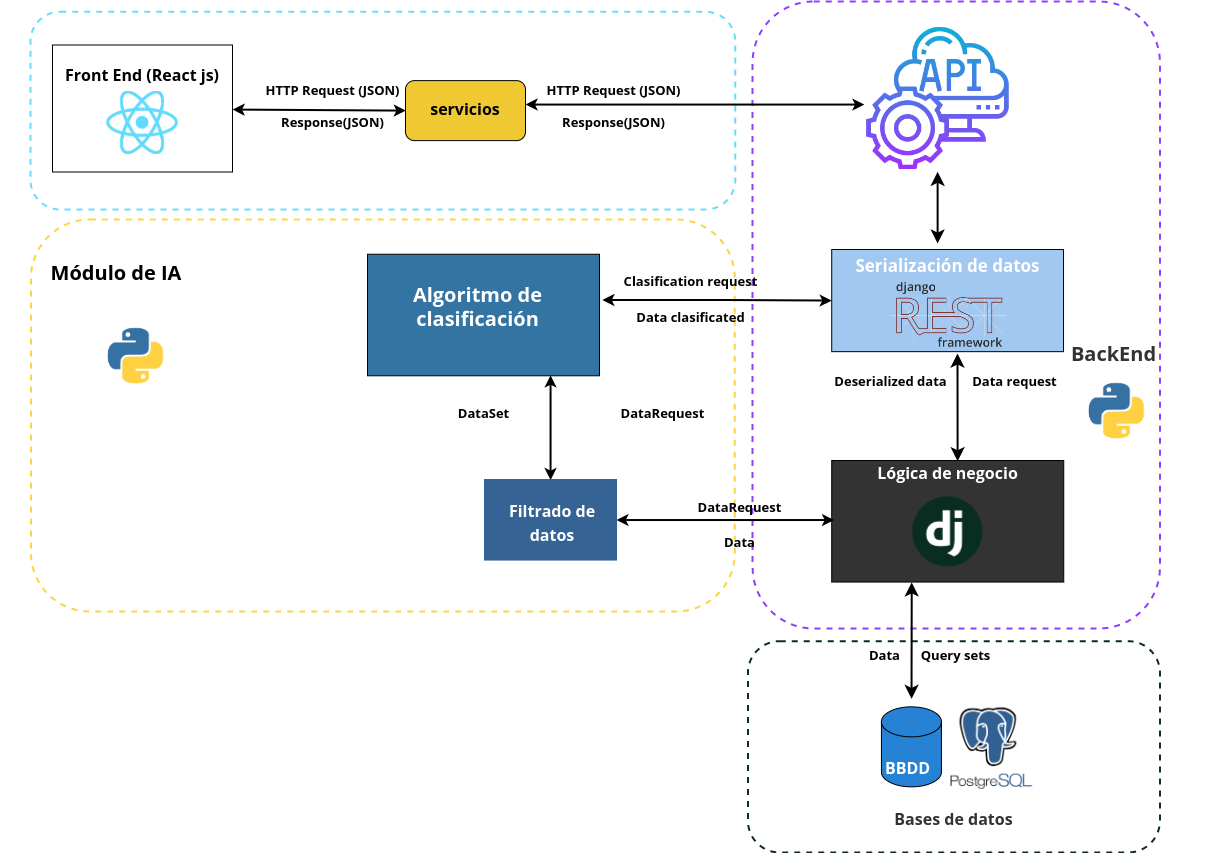
\includegraphics[width=.9\textwidth]{propuesta/imagenes/arqui.png}
    \end{center}
    \caption{Arquitectura del sistema}
    \label{fig:arquitectura}
\end{figure}


%\begin{description}
%    \item[Servidor Web] El servidor web es el punto de entrada a nuestra herramienta, en el se alberga el código HTML, 
%    CSS y JS compilado React Js.
    %\item[Bases de Datos] Cada servicio de nuestra arquitectura cuenta con su propia base de datos. Esto es para eliminar la dependencia entre ellos. Todas las bases de datos utilizan el gestor de Postgres debido a su eficiencia en desempeño y consultas además de que es open source.
%\end{description}